\chapter{Experimental method}

\paragraph{}
The state-decomposition method is going to be implemented and tested in multiple varieties to assess the effect it has when
applied to reinforcement learning algorithms. 

\section{Tools}

\paragraph{Python}
The programming language chosen for this project is Python. This is motivated by Python being a high-level language that allows
writing compact, readable code and by the widespread availability of resources and packages for it (such as the OpenAI Gym toolkit
previously described). Additionally, Python can be run on Colab notebooks.

\paragraph{Google Colaboratory}
Google Colab is a platform from Google which is widely used for machine learning research and prototyping of new models. Colab
combines a notebook platform that many Python developers are familiar with and the high-performance of cloud computing. The user
can choose to run a program using CPUs, GPUs, or TPUs\footnote{Tensor Processing Unit: a custom hardware accelerator developed by
Google to accelerate the linear algebra operations that occur in machine learning. \cite{noauthor_cloud_nodate}}. Examples of the
available GPUs are Nvidia K80 and NVidia P100D. The disadvantage of Colab compared to cloud computing platforms such as Google
Cloud and Amazon AWS is that the user is not guaranteed full access to the hardware accelerators (such as GPUs) and thus the
performance can vary. The session length is also limited to 12 hours. These problems are mitigated by purchasing a "Pro" license
for the price of \$10 per month, which prioritises access to GPUs and increases the maximum session length to 24 hours. The level
of performance offered by Colab Pro is enough for this project. The main advantage is an easy to use platform thanks to its
notebook format, rather than the less user-friendly access via SSH in the Terminal required by other cloud-computing platforms. 

\paragraph{Keras}
It was decided to implement the deep-learning models using the deep-learning API Keras \cite{keras}. This is a high-level
interface that uses Tensorflow \cite{noauthor_tensorflow_nodate} for its backend. Keras allows to code deep-learning models in a
very readable and compact way. Having Tensorflow as its backend, it can run on CPUs, GPUs, and TPUs, taking advantage of the
high-performance hardware offered by Google Colab.

\paragraph{OpenAI Gym}
As this project deals with the development and evaluation of a new method for reinforcement learning algorithms, it was decided to
apply it in a "toy environment" that would simplify experimentation. OpenAI offers an open-source Python toolkit called "OpenAI
Gym" \cite{openai_gym_nodate}, which is currently the most commonly used toolkit to benchmark reinforcement learning algorithms.
This toolkit offers a variety of different environments, ranging from classical control problems such as "CartPole-v0"
\cite{noauthor_openai_nodate}, to more complicated environments such as playing Atari games using the pixel data as sensory input
or solving robotic manipulation problems. The "OpenAI Gym" offers environments with a wide range of complexities and all
combinations of discrete and continuous state and action spaces.

\begin{figure}[H]
    \centering
    \includegraphics[width = 0.5\linewidth]{figures/cartpole.PNG}
    \caption{The CartPole-v1 environment is one of the most well-known environments of the OpenAI Gym library in which the goal is
    to balance the cartpole while keeping it within the boundaries of the screen by applying a leftwards or a rightwards force at
    each time-step. Screenshot of \cite{noauthor_openai_nodate}}
    \label{fig:cartpole}
\end{figure}

\section[Obtaining the state trans. matrix]{Obtaining the state transition matrix}

\paragraph{}
The first step in the state-decomposition method is to obtain the state-transition matrix. Since we are testing the algorithm in
software simulations, the state-transition matrix can be easily obtained from the source code of the environments and it can be
considered as given. This is usually not the case, so at a later stage we shall test methods to approximate the state-transition
matrix. This can be done by interacting with the environment and sampling the $\langle S,A,R,S' \rangle$ tuples that are
generated. Since the state-transition probabilities are dependent on the action, the state-transition matrix is dependent on the
chosen policy. As we are conducting this before the training and we have no information about the optimal policy, we choose to use
the most general possible policy to obtain the state-transition table, that is, the actions are all chosen with equal probability
independently of the current state. The number of iterations required to construct the state-transition matrix is dependant on the
number of states, actions, the probability of visiting each different state and the required level of accuracy of the
state-transition matrix estimate. 

\section{The need for a suitable environment} \label{sec:TaxiTraps}

\paragraph{}
The state-transition matrices and their decomposed versions were obtained for 4 different OpenAI Gym environments:
"Cartpole-v1"\footnote{This environment has continuous states which are discretised using a linear quantiser to apply the
decomposition algorithm.}, "FrozenLake8x8-v0", "CliffWalking-v0" and "Taxi-v3". The state-decomposition algorithm is aimed at
environments whose state-spaces decompose into similarly sized sub-spaces, as this is the case in which the method would be
potentially very effective. If one of the state-spaces is much greater than the others and similar in size to the original
state-space, the reduction in complexity of the training in the first stage would not compensate for the more complex multi-stage
nature of the state-decomposition method. Having sub-spaces that are too small (in the extreme case having just one state) limits
the amount of learning that can be achieved in the first stage of training, simply delaying this to the second stage. The MDPs of
"Cartpole-v1", "FrozenLake8x8-v0", "CliffWalking-v0", always decompose into one big sub-space and sub-spaces formed by only one
state. This occurs because these environments are not formed of almost independent sub-problems that rarely interact with each
other. 

\paragraph{}
The "Taxi-v3" environment, shown on the left in Figure-\ref{fig:taxi} is a more suitable candidate. The environment presents:
\begin{itemize}
    \item 500 discrete spaces, corresponding to 25 taxi positions in the 5x5 grid, 4 possible destinations, and 5 possible
    passenger positions (1 of which is inside the taxi).
    \item 6 discrete actions: 4 moves (up, down, left, right), pick-up passenger, and drop-off passenger.
    \item Rewards: +20 for a successful drop-off, -1 at each time step (also when hitting a wall), and -10 for illegal pick-up and
    drop-off actions.
\end{itemize}

An episode terminates when the passenger is successfully dropped off or after 200 time-steps. Applying the state-decomposition to
this environment can form 4 equally sized sub-spaces even with a threshold of 0, meaning that these are 4 completely independent
sub-spaces that can be treated as independent Markov Decision Processes. These 4 sub-spaces correspond to the 4 possible
destinations of the passenger, which never change during a single episode. Thus, this a more specific and easier problem than the
one we are trying to solve, where the subsystems, though rarely, do interact with each other. Thus, this environment is not
suitable for testing the state-decomposition algorithm as good performance of the algorithm in this simpler environment does not
imply good performance in the more general scenario. 

\paragraph{}
These problems in finding a suitable environment suggest that the best solution would be to create a custom environment with the
characteristics that would allow better testing of the method. The "Taxi-v3" environment is composed of 4 independent MDPs.
Modifying its transition-probabilities so that interaction between them is possible\footnote{Making transition-probabilities
between spaces of different subsystems non-zero.}, would make this environment suitable for testing the decomposition algorithm.
For this purpose, I propose a modified version called "TaxiTraps", with added "traps" located on the edges of certain squares.
These activate with a low probability $p_{trap}$ when the Taxi moves over them. If a trap does not activate, the taxi simply moves
over it as in the original "Taxi-v3" environment. When the trap does activate, the behaviour of the environment is modified in two
ways:

\begin{enumerate}
    \item The destination of the Taxi changes. This makes it possible for the destination of a passenger to change during an
    episode, thus providing the transitions between different sub-spaces that exist in the general problem that the
    state-decomposition method is aimed at.
    
    \item A highly negative reward is released. This was added to ensure that the optimal policy in the "TaxiTraps" environment is
    different than in the original Taxi environment. Since in the first step of the state-decomposition method the transitions
    between different state sub-spaces are ignored, the agents are trained in an environment equivalent to the original "Taxi-v3".
    If the optimal policy is the same in "Taxi-v3" and "TaxiTraps", the optimal policy would not change between the first and
    second training stage of training, which is unlikely to happen in a general scenario. Thus, ensuring that the optimal policy
    changes between training stages is required for the results of testing to generalise to other environments.  
\end{enumerate}

%Is the fact that we are discouraging the Taxi to go over the traps a problem as in the final policy we are kind of ignoring
%transitions because we actively avoid them?

\begin{figure}[H]
\centering
    \resizebox{\linewidth}{!}{
    \subfloat["Taxi"]{
        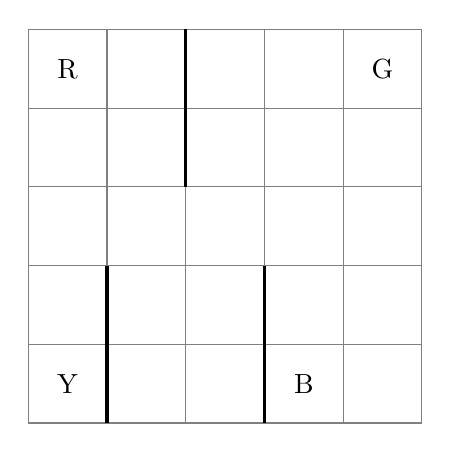
\begin{tikzpicture}
            \draw[step=1cm,color=gray] (0,0) grid (5,5);
            \node at (0.5,4.5) {R};
            \node at (4.5,4.5) {G};
            \node at (0.5,0.5) {Y};
            \node at (3.5,0.5) {B};
            \draw[very thick] (2,5) -- (2,3);
            \draw[very thick] (1,2) -- (1,0);
            \draw[very thick] (3,2) -- (3,0);
        \end{tikzpicture}}
    \qquad
    \subfloat["TaxiTraps"]{
        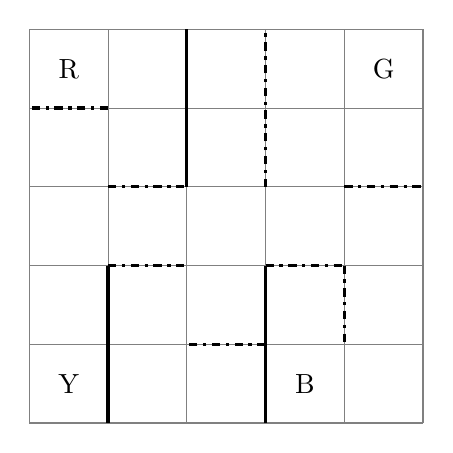
\begin{tikzpicture}
            \draw[step=1cm,color=gray] (0,0) grid (5,5);
            \node at (0.5,4.5) {R};
            \node at (4.5,4.5) {G};
            \node at (0.5,0.5) {Y};
            \node at (3.5,0.5) {B};
            \draw[very thick] (2,5) -- (2,3);
            \draw[very thick] (1,2) -- (1,0);
            \draw[very thick] (3,2) -- (3,0);
            \draw[very thick, dash dot] (1,4) -- (0,4);
            \draw[very thick, dash dot] (1,3) -- (2,3);
            \draw[very thick, dash dot] (3,1) -- (2,1);
            \draw[very thick, dash dot] (1,2) -- (2,2);
            \draw[very thick, dash dot] (3,2) -- (4,2);
            \draw[very thick, dash dot] (4,3) -- (5,3);
            \draw[very thick, dash dot] (3,3) -- (3,5);
            \draw[very thick, dash dot] (4,2) -- (4,1);
        \end{tikzpicture}}
    \qquad
    \subfloat["Taxi2"]{
        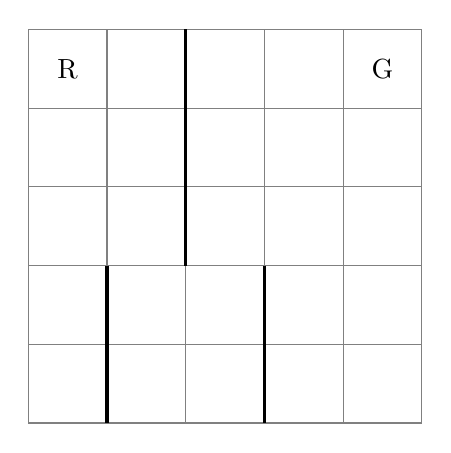
\begin{tikzpicture}
            \draw[step=1cm,color=gray] (0,0) grid (5,5);
            \node at (0.5,4.5) {R};
            \node at (4.5,4.5) {G};
            \draw[very thick] (2,5) -- (2,3);
            \draw[very thick] (1,2) -- (1,0);
            \draw[very thick] (3,2) -- (3,0);
            \draw[very thick] (2,3) -- (2,2);
        \end{tikzpicture}}}
    \caption{Original and modified 'Taxi' environments. The thick black lines represent the walls, while the dotted lines represent the "traps".}
    \label{fig:taxi}
\end{figure}

\section{Implementation of the DQN agents}

Some initial testing of the state decomposition method has been conducted in the "Taxi-v3" environment. Here, the
state-decomposition method modified to skip the second stage of joining the networks together showed equivalent performance as a
single DQN agent. The equivalence is to be expected since in this environment the sub-problems are completely independent and it
does not prove anything about the algorithm in general. One issue of the testing conducted until now is the format in which the
states were fed into the Neural Networks. The OpenAI Gym library represents discrete states and actions as single integers. Such a
representation is optimal when using tabular Q-learning, as the representations of states and actions simply act as indexes and
don't need to be meaningful. However, when using a Q-function approximator, such a meaningless representation impedes the
generalisation properties in unseen states that make DQN so useful. Representing the states as one-hot encoded versions of the
original integer has also been tested. Though this could allow using shallower neural networks as the decoding of the states is
simpler, this is still not a meaningful representation of the states. The current state of the code of the state-decomposition
agent is given in the Appendix. To take full advantage of the generalisation to unseen states property of DQN, the format in which
states are input to the agents will be modified to be a meaningful representation. This could be in a vector format, where each
element of the vector represents a different aspect, such as position, destination, etc.

\section{Benchmark DQN agent}

The aim of this project is to determine whether state-decomposition techniques can be used to increase the efficiency of
reinforcement learning algorithms. Doing so requires comparing the performance of an algorithm where state-decomposition was
applied and that of the same algorithm without state-decomposition, while choosing all other parameters to be the same or to be
the values hat make for the fairest comparison. The number of possible choices to be made in these algorithms is such that
providing a fair comparison can be a non-trivial task, as discussed in the following section. 

The chosen benchmark agent is a basic DQN agent. The value updates occur with discount factor $\gamma=0.95$ WHY??? (I think even
though the episode are finite so could use gamma=1, using a lower gamma enhaces the stability of the algorithm). The agents acts
according to an $\epsilon$-greedy policy. This means that at each agent-environment interaction, the agent picks the value that
currently has the highest estimated action value with probability $1-\epsilon$ or a random action with probability $\epsilon$
(RANDOM OR ONE OF THE OTHERS? NOt big difference anyways). $\epsilon$ is initialised at 1, meaning that in the first iteration the
action is completely random and decays by a factor $0.999$ after each update of the action values. $\epsilon$ is set to stop
decreasing at $\epsilon=0.01$, this is to ensure that the algorithm doesn't stop exploring by having too small an $\epsilon$. 

The neural network that approximates the Q-values is fully connected and it has 4 layers. The input state is fed as an integer to
an encoding layer\footnote{This is fixed and pre-programmed and doesn't include any learned parameters.}, which then feeds to the
first fully-connected layer, consisting of 512 neurons with "ReLU"\footnote{"ReLU" stands for Rectified Linear Unit. It represents
the function $f(x)=\max(0, x)$. Neural networks rely on the non-linear activation functions such as "ReLU" in order to be able to
learn non-linear functions.} activation function. This is then followed by 2 similar layers, having 256 neurons each. The last
layer consists of a number of neurons corresponding to the number of actions in the environment where the agent is being used.
Each output of the network corresponds to the action value of an action, thus the activation function was chosen to be linear,
that is, the outputs of the layer are equal to the outputs of the neurons. This is to allow the outputs to take any possible
values, without upper or lower bounds so that the network is theoretically capable of mapping any state to any possible
action-value. The network is updated using "Minimum Square Error" as its loss function, that is, at each update step, the network
weights are updated to reduce the function $L = \sum_{i=1}^n (y_i-f_{\theta}(x_i))^2$ where $x_i$ are the inputs, $y_i$ the
corresponding outputs and $f_{\theta}$ is the function implemented by the neural network with weights $\theta$. 